%%%%%%%%% MASTER -- compiles the 4 sections

\documentclass[11pt,a4paper]{article}
\usepackage[margin=1in,footskip=0.5in]{geometry}


%%%%%%%%%%%%%%%%%%%%%%%%%%%%%%%%%%%%%%%%%%%%%%%%%%%%%%%%%%%%%%%%%%%%%%%%%
\pagestyle{plain}                                                      %%
\newcommand{\required}[1]{\section*{\hfil #1\hfil}}                    %%
\renewcommand{\refname}{\hfil References Cited\hfil}                   %%
\bibliographystyle{plain}                                              %%
%%%%%%%%%%%%%%%%%%%%%%%%%%%%%%%%%%%%%%%%%%%%%%%%%%%%%%%%%%%%%%%%%%%%%%%%%

%PUT YOUR MACROS HERE
\usepackage{comment}
\usepackage{graphicx}
\usepackage{wrapfig}%%
\usepackage{caption}
\usepackage{subcaption}
\usepackage{array}
\usepackage{booktabs}
\usepackage{amsmath} % assumes amsmath package installed
\usepackage{amssymb}  % assumes amsmath package installed
\usepackage[pageanchor=true,plainpages=false, pdfpagelabels, bookmarks,bookmarksnumbered,hidelinks]{hyperref}
\usepackage{bookmark}
\usepackage{framed}
\usepackage{url}
\usepackage{color,soul}
\usepackage{sidecap}
%\includeonly{NSFsumm}
\usepackage{todonotes}
\usepackage{wasysym}  
\usepackage{enumitem}
\usepackage{tabularx}
\usepackage{listings}
\usepackage{units}
\setlength{\parskip}{1em}
\newcolumntype{C}{>{\centering\arraybackslash}X}
\DeclareMathOperator*{\argmin}{arg\,min}
\DeclareMathOperator*{\argmax}{arg\,max}

\renewcommand{\bottomfraction}{0.8}
\renewcommand{\textfraction}{0.2}
\newcommand\notes[1]{{\noindent\color{blue}#1}}

\graphicspath{{figures/}}

\newenvironment{packed_item}{
  \setlength{\partopsep}{-8pt}
  \begin{itemize}
  \setlength{\itemsep}{1pt}
  \setlength{\parskip}{0pt}
  \setlength{\parsep}{0pt}
}{\end{itemize}}

\newenvironment{packed_enum}{
  \setlength{\partopsep}{-8pt}
  \begin{enumerate}
  \setlength{\itemsep}{1pt}
  \setlength{\parskip}{0pt}
  \setlength{\parsep}{0pt}
}{\end{enumerate}}

\newenvironment{checklist}{
  \setlength{\partopsep}{-4pt}
  \begin{packed_item}
  \let\olditem\item
  \renewcommand\item{\olditem[$\Box$] }
  \newcommand\checkeditem{\olditem[$\CheckedBox$] }
}{\end{packed_item}}   

\newcommand{\draftnote}[1]{\marginpar{\tiny\raggedright\textsf{\hspace{0pt}#1}}}
\linespread{0.995}

\newcommand{\PropTitle}{CROWDBOT: Pepper Control and Planning\\ \small{ETH Z\"{u}rich}}
\begin{document}
\setcounter{page}{1}
\section*{\PropTitle}
\vspace{-0.5cm}
\rule{\textwidth}{0.05cm}
\vspace{0.5cm}
\begin{abstract}
This report details the control behaviors of the Pepper robot. It provides an analysis of the platform response to input commands from a joypad controller. The findings in this report should be used as guidelines for designing planning and navigation algorithms for the Pepper platform.
\end{abstract}

\section{Experimental Setup} \label{sec:setup}

\begin{figure}[h]
\centering
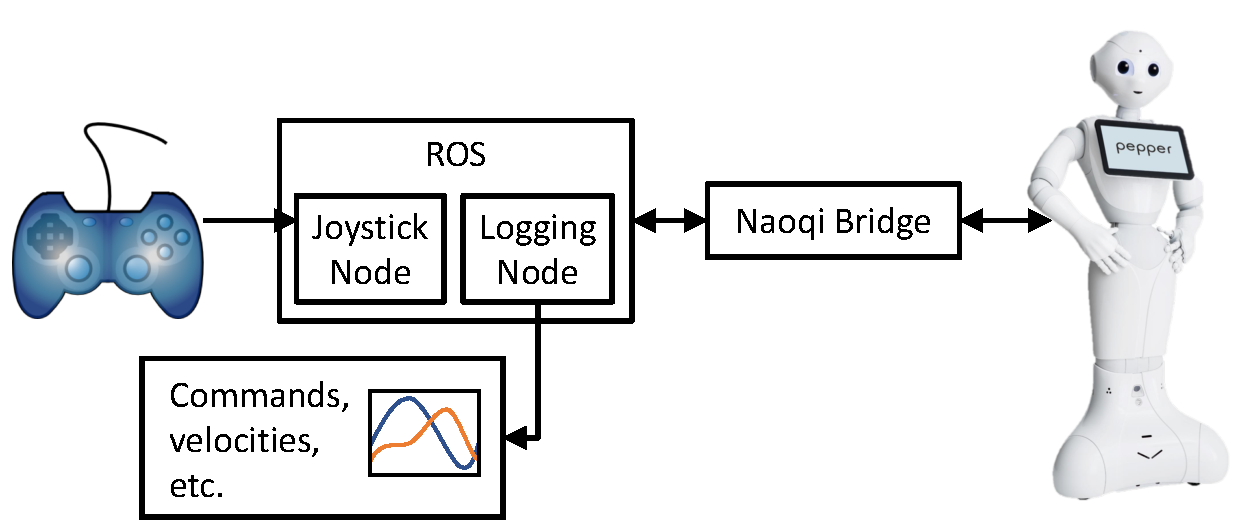
\includegraphics[width=0.7\textwidth]{figures/pepper_control.pdf}
\caption{The control response of the Pepper robot was tested through a joypad controller. Commands from the joypad were interpreted by the ROS joystick node which interfaces with the NAOqi bridge to the platform.} \label{fig:pepper_control}
\end{figure}

During the experiment, the Pepper robot was controlled through the ROS interface, specifically the open source naoqi\_driver ROS package. Commands from the joystick device were transmitted through ROS messages to the naoqi\_driver ROS node running on an offboard PC. naoqi\_driver in turn converted ROS messages to ALMotion commands, according to the NAOqi API. The ALMotion commands were then transmitted through ethernet connection to the Pepper onboard computer, where the running NAOqi OS executed them.

The joystick was set to a variable refresh rate, with a minimum of 2Hz and maximum of 100Hz. Changes in the value of an axis or button state immediately trigger a corresponding motion command (within the maximum rate limit), whereas in the abscence of changes in axis or button values, the last motion command is repeated at a rate of 2Hz.

For motion testing, Pepper was placed in a large room with no obstacle and on soft, grippy surfaces where no significant wheel slip was observed.

Additionally, during all testing, the NAOqi anti-collision safety protocols where disabled. The following autonomous abilities were disabled as well: AutonomousBlinking, BackgroundMovement, BasicAwareness, ListeningMovement, SpeakingMovement. 

\subsection{Tests} \label{sec:tests}

The following tests cases are carried out in order to quantify the control envelope of the Pepper robot:

\begin{packed_enum}
\item Maximum forward acceleration to top speed.
\item Maximum reverse acceleration from top forward speed to top reverse speed.
\item Maximum side acceleration to top speed.
\item Maximum side acceleration from top speed to top speed in opposite direction.
\item Stopping from top forward speed with killMove command.
\item Stopping from top side speed with killMove command.
\item Maximum reverse acceleration from top forward speed to top reverse speed using killMove. 
\end{packed_enum}

During testing, delays are dissected as far as possible into their components and causes, in order to evaluate the influence of various parts of the pipeline responsible on latency.

\section{Results} \label{sec:results}

\subsection{Command Propagation}

Command propagation times are measured with varying levels of certainty. Delays within pepper itself are only inferred based on the measured outputs, whereas delays due to ROS or ethernet transmission can be measured directly. It should be noted for example that the ROS-induced delay variance is dominated by variance in measured values whereas the NAOqi OS delay variance is dominated by uncertainties in our model of the underlying process, and indirectness of measured values.

\begin{lstlisting}[frame=single, caption={Example output for network latency measurements}]
daniel@prometheus:~ $ ping 172.30.50.11
PING 172.30.50.11 (172.30.50.11) 56(84) bytes of data.
64 bytes from 172.30.50.11: icmp_seq=1 ttl=64 time=0.286 ms
64 bytes from 172.30.50.11: icmp_seq=2 ttl=64 time=0.296 ms
64 bytes from 172.30.50.11: icmp_seq=3 ttl=64 time=0.277 ms
64 bytes from 172.30.50.11: icmp_seq=4 ttl=64 time=0.320 ms
64 bytes from 172.30.50.11: icmp_seq=5 ttl=64 time=0.265 ms
64 bytes from 172.30.50.11: icmp_seq=6 ttl=64 time=0.278 ms
64 bytes from 172.30.50.11: icmp_seq=7 ttl=64 time=0.325 ms
...
\end{lstlisting}

\begin{table}[h]
  \centering
  \caption{Command propagation times}
  \label{tab:command_time}
  \begin{tabular}{ l  l  c }
  \toprule
   From & To & Delay [ms] \\\midrule
   Joystick actuation registration & moveToward command emission &  $20 \pm10$ \\
   moveToward command emission & Reception NAOqi OS (LAN) &  $0.3 \pm0.03$\\
   Reception NAOqi OS & Servo actuation & $100 \pm50$ \\\bottomrule
  \end{tabular}
\end{table}

\subsection{Pepper Velocity Response}

Velocity response measurements are extracted from NAOqi OS odometry, however their accuracy is not well known. Further testing with external sensors would be necessary in order to acquire a more precise estimate of the velocity response. The response times measured in the velocity tests were however large enough ($\unit[1\times10^3]{ms}$) that they dominate over estimated measurement bias and standard deviation ($\unit[1\times10^2]{ms}$).

The acceleration profile average times presented in Table~\ref{tab:acc_profiles} are measured from the start of servo actuation to the realization of target velocity. The exact point for realization is not straightforward to define. We define it as being $\unit[50]{ms}$ before the first inversion of the velocity derivative within $0.95v_{max} - v_{max}$.
For values corresponding to tests 1 to 6 in Table~\ref{tab:acc_profiles}, uncertainty was estimated be in the order of $\unit[100]{ms}$, composed of i) uncertainty in the propagation time from joystick to servo actuation, ii) variance due to odometry data noise, iii) variability of the target velocity realization condition.

\begin{figure}[h]
\centering
\text{Velocity response example}
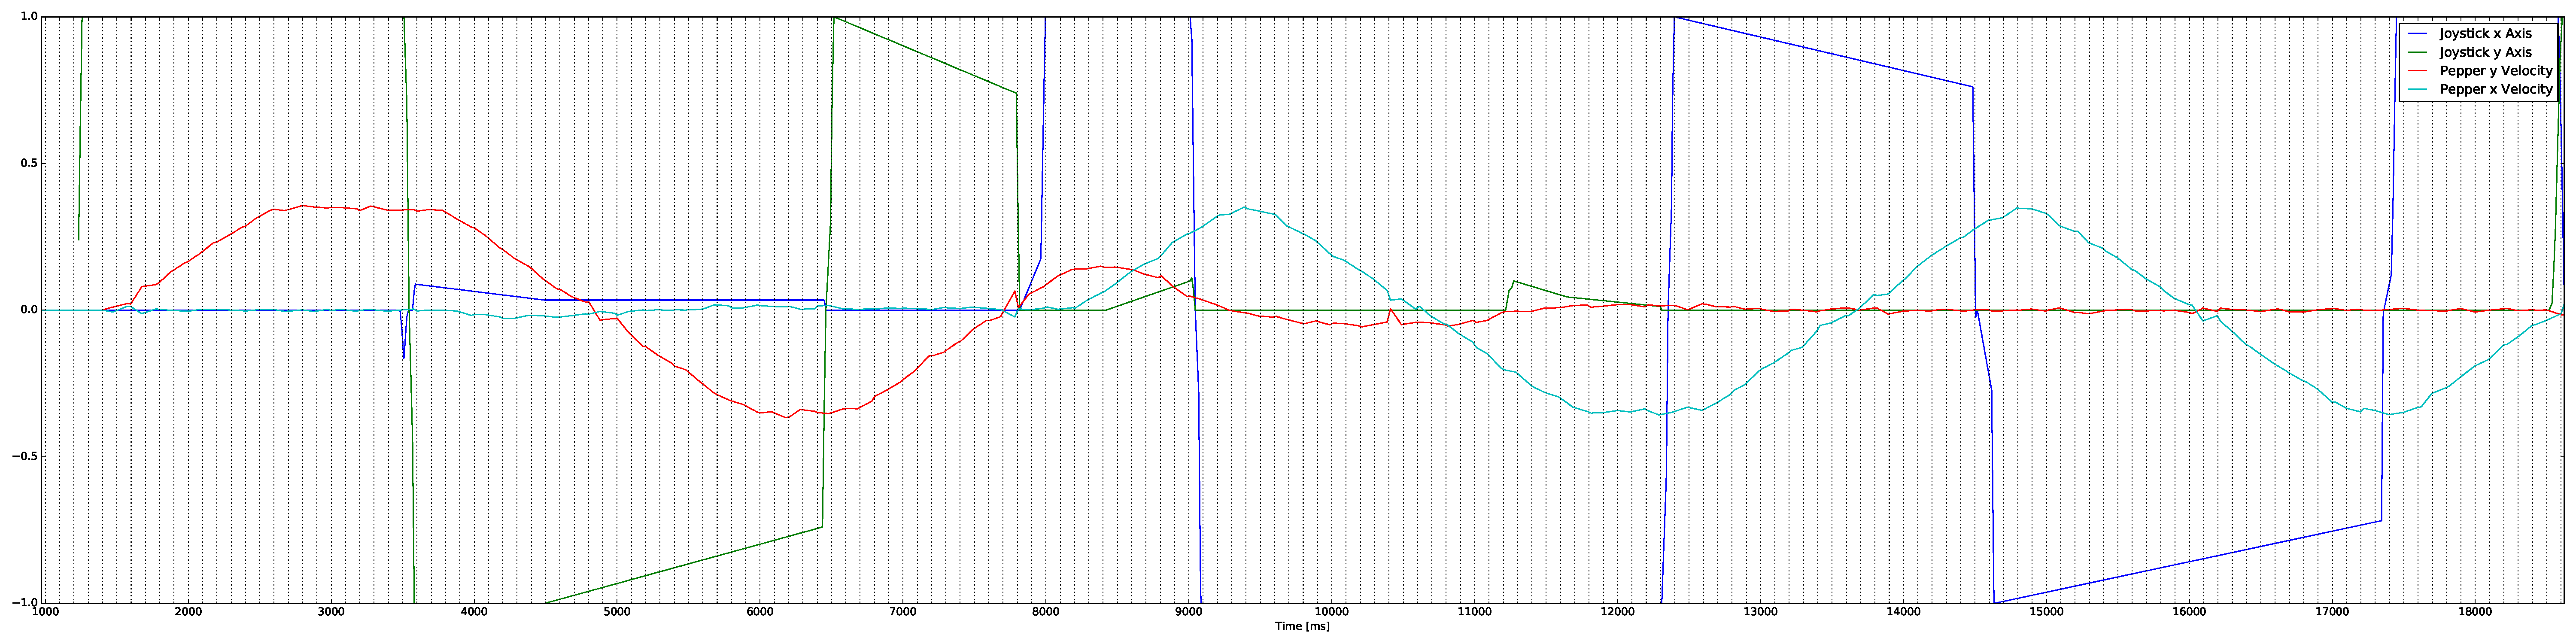
\includegraphics[width=1\textwidth]{figures/PepperPerformance.pdf}
\caption{Pepper velocity measurements compared to moveToward commands from the joystick, including forward-back, and side-to-side movement. Velocities are in [m/s], moveToward commands are unitless [0, 1]. Commands were transmitted from the joystick ROS node to NAOqi OS via naoqi\_driver and ethernet. The joystick (x,y) commands are plotted in blue and green, respectively. The measured (x,y) velocities are plotted in cyan and red, respectively.}
\label{fig:xy_performance}
\end{figure}

\begin{table}[h]
  \centering
  \caption{Acceleration profiles}
  \label{tab:acc_profiles}
  \begin{tabular}{ l  c  c }
  \toprule
   Test set & Average time $[s]$ \\\midrule
   1. $v=0$ to forward $v_{\mathit{max}}$ & 1.3  \\
   2. forward $v_{\mathit{max}}$ to backward $v_{\mathit{max}}$ & 2.4  \\
   3. $v=0$ to side $v_{\mathit{max}}$ & 1.3  \\
   4. side $v_{\mathit{max}}$ to opposite side $v_{\mathit{max}}$ & 2.4  \\
   5. forward $v_{\mathit{max}}$ to $v=0$ with killMove & 0.9  \\
   6. side $v_{\mathit{max}}$ to $v=0$ with killMove & 0.9  \\
   7. forward $v_{\mathit{max}}$ to backward $v_{\mathit{max}}$ with killMove & 1.9 - 2.4  \\\bottomrule
  \end{tabular}
\end{table}

\subsection{killMove Command Acceleration Characteristics}\par

For the purpose of testing, the joystick was configured to emit the killMove ALMotion command upon button press. The recorded servo accelerations when executing the killMove command are demonstrably higher than the maximum acceleration values attainable through the ALMotion moveToward command. No toppling over or unstable behavior was observed during the killMove maneuver.


\begin{figure}[h]
\centering
\text{Response to killMove command in forward/backward directions}
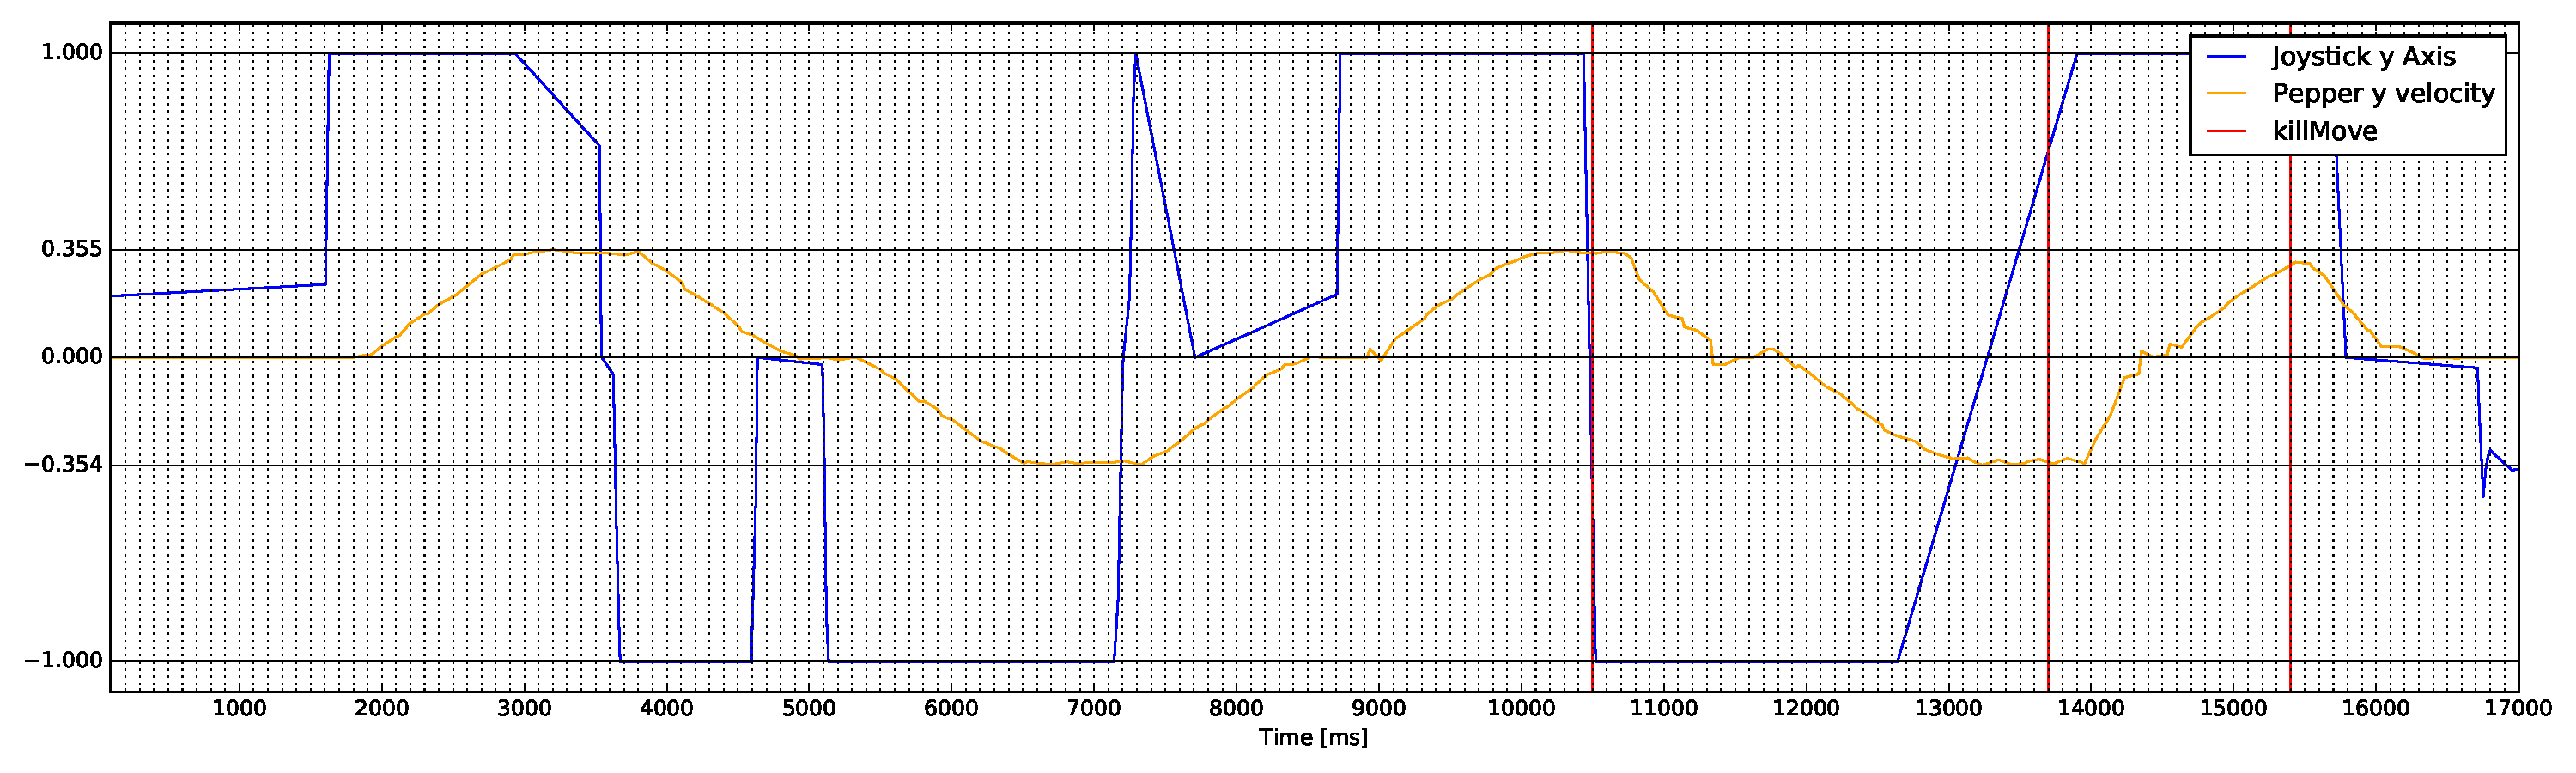
\includegraphics[width=1\textwidth]{figures/kill_move_forwardback_pepper_performance.pdf}
\caption{Comparison in velocity responses with and without using the killMove command. Velocities are in [m/s], moveToward commands are unitless [0, 1].} 
\label{fig:killmove_forwardback_performance}
\end{figure}

\begin{figure}[h]
\centering
\text{Response to killMove command in sideways directions}
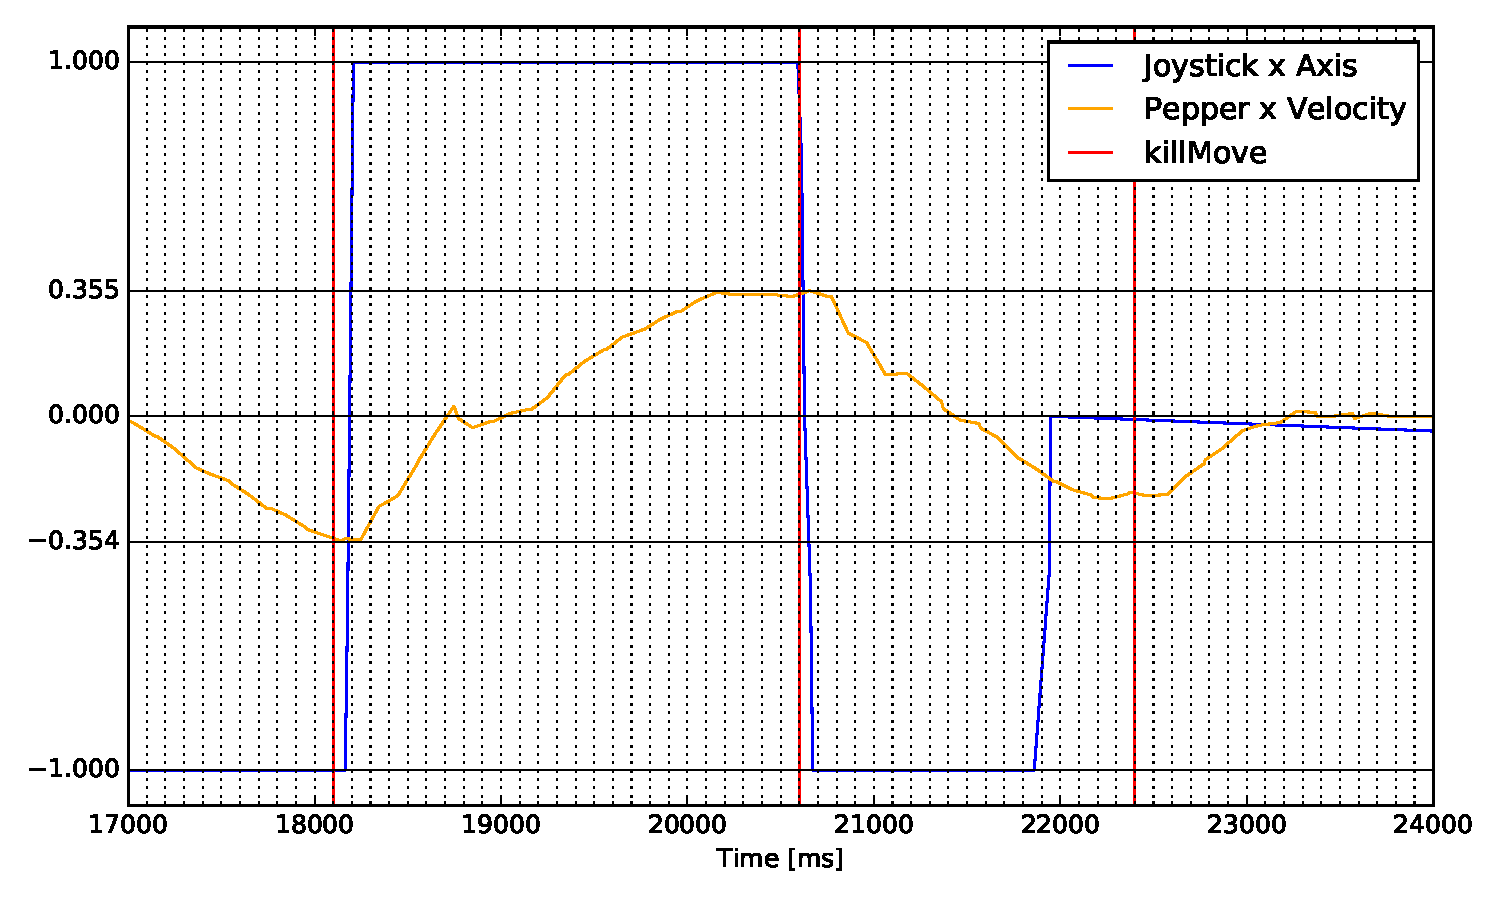
\includegraphics[width=0.5\textwidth]{figures/kill_move_side_pepper_performance.pdf}
\caption{killMove command applied to sideways velocities. Velocities are in [m/s], moveToward commands are unitless [0, 1].} 
\label{fig:killmove_side_performance}
\end{figure}

\section{Analysis and Recommendations for Planning}

The exact wheel control properties and design of NaoqiOS are largely unknown. Based on the measurements described in Section~\ref{sec:results}, we speculate the following:


The shape of the velocity measurements shows smooth changes in velocity, which would seem to indicate that the NAOqi OS wheel controller enforces linear jerk/constant snap constraints. This hypothesis is further reinforced when comparing acceleration times for i) max velocity to stop, and ii) max velocity to min velocity. The measured time for case i) takes on average $\unit[100]{ms}$ longer than that of case ii). If acceleration was simply mapped linearly to joystick axis for example, and set to 0 when the target velocity was reached, we would expect the delay in case i) to be exactly half that of case ii). If linear jerk is enforced however, the necessary reduction of acceleration when approaching the target velocity leads to additional delay in reaching the target velocity.


Based on the maximum accelerations measured using the i) killMove and ii) moveToward, it would seem that the NAOqi OS sets conservative limits on maximum acceleration during normal operation which can only be exceeded in exceptional scenarios (killMove). One consequence is that using maximum values for the moveToward Pepper control is not only safe, but almost always recommended, as its use does not approach in any way the mechanical and kinematic limits of the robot.


The possibility of using killMove not only for stopping, but also for changing direction as quickly as possible, was a point of interest. However, even though the command leads to higher deceleration than otherwise, there is a significant variable delay after its use before the robot starts executing movement commands again. In our tests, this delay often negated the gains achieved from using the command for this purpose. Furthermore, in our use case, predictability of command completion-time is strongly desired. As such, using killMove for direction changes is not currently advisable. However, we could foresee this conclusion being invalidated in the future, as a better understanding of the internal NAOqi processing of motion commands might lead to the discovery of solutions for the unpredictability issue.


The moveTo command was not tested as thoroughly as the moveToward command. In all our tests however, the resulting acceleration of the robot was never observed to be greater than with the moveToward command. A rough, qualitative evaluation seemed to indicate that the delay between executing successive commands using the moveTo command was less predictable and often greater than with the moveToward command. As such we have opted for use of the moveToward command for control in dynamic environments. In our limited experience, for waypoint-based navigation in static environments, the moveTo command remains suitable.

The effect of the motion command rate, in our case related to the joystick refresh rate, on the motion properties of Pepper were not properly examined in the scope of this project. However, as visible on Figure~\ref{fig:joystick_rate}, the effect of command rate on the control behavior are not observed to be significant.

\begin{figure}[h]
\centering
\text{Variable joystick rate visualized}
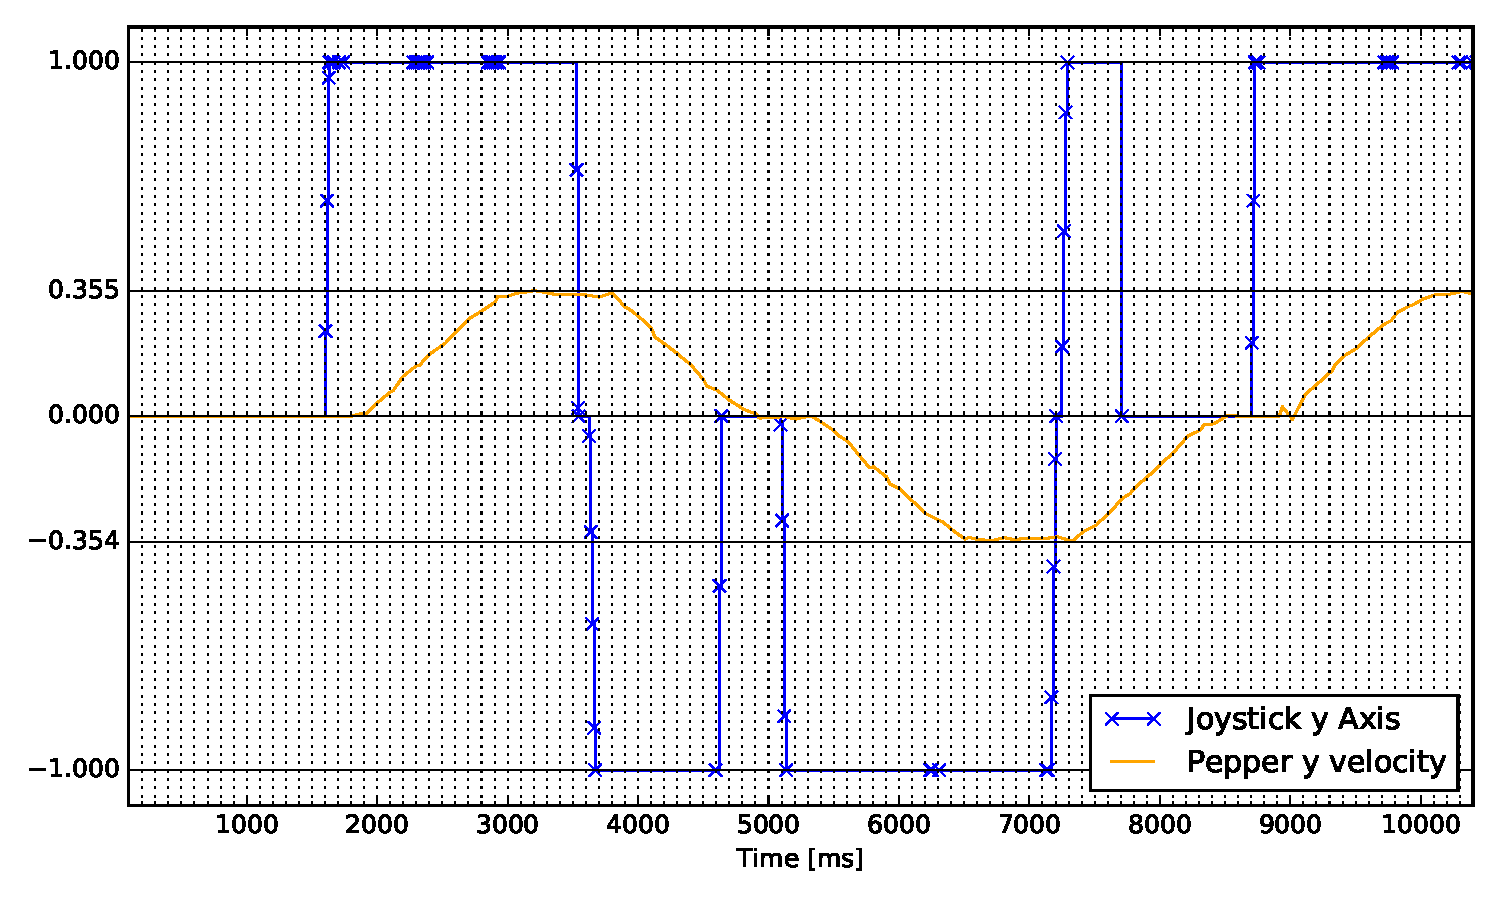
\includegraphics[width=0.8\textwidth]{figures/variable_joystick_rate.pdf}
\caption{In this figure, each time where a command is labeled with an x marker. Velocities are in [m/s], moveToward commands are unitless [0, 1].} 
\label{fig:joystick_rate}
\end{figure}

\end{document}